
\usepackage[utf8x]{inputenc}
\usepackage{ucs}
\usepackage{amsmath}
\usepackage{amsfonts}
\usepackage{amssymb}
\usepackage{multicol}
\usepackage{graphicx}
%\usepackage{hyperref}		% automatic included by beamer
\usepackage{tikz}
\usetikzlibrary{arrows,positioning,shapes}
\usepackage{listings}
\usepackage{multicol}
\usepackage{appendixnumberbeamer}
\usepackage{pstricks}
\usepackage{marvosym}

\title{perf}
%\subtitle{}
\author{Urs F\"assler}
\date{14.07.2011}
\institute
{
  CERN Openlab
}
%\subject{}

\lstset
{  
  basicstyle=\small\ttfamily,
  language=,
  morekeywords={interface,function,query,String,Integer,Boolean,component,import,input,output,implementation,connection,elementary,hfsm,state,initial,entry,exit,var,do,end,true,false,return,transition,to,by,if,ef, then,else},
  comment=[l]{//},
  morecomment=[s]{/*}{*/},
%  numbers=left,
  numberstyle={\color{Grey}},
  keywordstyle={\bfseries\color{DarkRed}},
%  identifierstyle={\color{Blue}},
%  columns=flexible,
  float=tb,
  frame=single,
  escapeinside={@}{@},
  breaklines=true, % sets automatic line breaking
  breakatwhitespace=false % automatic breaks happen at whitespace
}

\bibliographystyle{plain}

\usetheme{Madrid}
\beamertemplatenavigationsymbolsempty

\begin{document}
\begin{frame}[plain]
  \titlepage
\end{frame}

\setcounter{framenumber}{0}

\begin{frame}{architecture (1)}
\centering{
  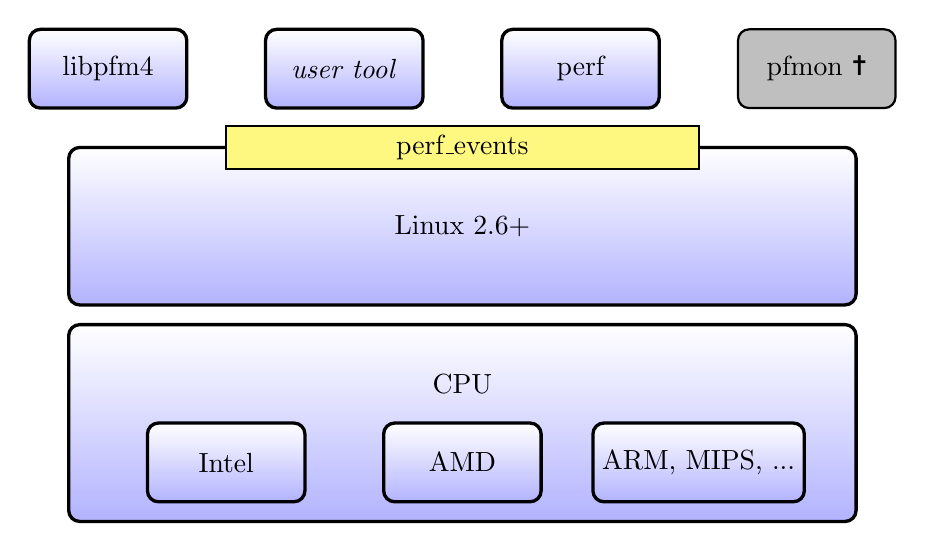
\begin{tikzpicture}[scale=1,transform shape]
\tikzstyle{size}=[minimum width=2 cm, minimum height=1 cm,anchor=center]

\tikzstyle{module}=[size,rectangle,rounded corners,draw=black, top color=white, bottom color=blue!30,very thick, text centered]
\tikzstyle{interface}=[rectangle,draw=black, fill=yellow!50,thick, text centered]
\tikzstyle{label}=[size,rectangle,text centered]

\node [module,minimum width=10 cm,minimum height=2.5 cm] at (0,0.5) (cpu)  {};
\node [label] at (0,1) (cpuLabel) {CPU};
\node [module] at (-3,0) (intel)  {Intel};
\node [module] at (0,0) (amd) {AMD};
\node [module] at (3,0) (arm) {ARM, MIPS, ...};

\node [module,minimum width=10 cm,minimum height=2 cm] at (0,3) (linux)  {Linux 2.6+};

\node [interface,minimum width=6 cm] at (0,4) (perf)  {perf\_events};

\node [module] at (-4.5,5) (libpfm4)  {libpfm4};
\node [module] at (-1.5,5) (user)  {\textit{user tool}};
\node [module] at (1.5,5) (perf)  {perf};
\node [size,rectangle,rounded corners,draw,thick,fill=gray!50] at (4.5,5) (pfmon)  {pfmon \Cross};

\end{tikzpicture}
}
\end{frame}

\begin{frame}{architecture (2)}
\begin{description}
  \item[perf] profiler tool for Linux
  \item[perf\_events] Linux kernel Interface
  \item[libpfm4] helper library to map event names to event encoding
  \item[pfmon, perfmon] predecessor, development stopped\only<handout>{\cite{pfmon2007}}
\end{description}
\end{frame}

What are the limitations of the tools/components? 

\begin{frame}{perf\_events\only<handout>{\cite{kernel.org2011,Eranian2010}}}
\begin{itemize}
  \item abstraction of hardware
  \item based on file descriptors
  \item hardware events (performance counters, ...)
  \item software events (kernel)
\end{itemize}
\end{frame}

\begin{frame}{perf tool\only<handout>{\cite{Eranian2010}}}
\begin{itemize}
  \item included in kernel source tree (tools/perf)
  \item support for per-thread, per-cpu counting, sampling, tracing
  \begin{itemize}
    \item cmdline tool, curses-based gui
    \item operate like git: perf command arguments
  \end{itemize}
  \item profiling support similar to Oprofile
  \begin{itemize}
    \item collection $\Rightarrow$ perf record $\Rightarrow$ binary output file
    \item high level analysis $\Rightarrow$ perf report
    \item source level analysis $\Rightarrow$ perf annotate
    \item remote collect, local analysis possible
  \end{itemize}
  \item top-like mode $\Rightarrow$ perf top
\end{itemize}
\end{frame}

\begin{frame}{collection capabilities}
I would like you to discuss the technical details surrounding:
\begin{itemize}
  \item what can be collected?
  \item How is it done?
  \item Is the data accurate?
  \item To what extent?
\end{itemize}
\end{frame}



\begin{frame}{storing and presentation}
data storing and presentation capabilities (  Text output? Graphics? )
\begin{itemize}
  \item in which way is the collected data stored?
  \item How is it presented? (Text output? Graphics?)
  \item Etc + examples
\end{itemize}
\end{frame}

\begin{frame}{analysis capabilities}
in which ways can we look at the data and how are those ways relevant or useful for software or hardware benchmarking
\end{frame}

\begin{frame}{more information}
\begin{itemize}
  \item Homepage of Vince Weaver: perf\_events, accuracy and more\only<handout>{\cite{Weaver2011}}
    \url{http://web.eecs.utk.edu/~vweaver1/}
\end{itemize}
\end{frame}

\appendix
\section{Appendix}

\begin{frame}{Analyze virtualized machine}
\code{perf} has support for the Kernel-based Virtual Machine (KVM \cite{kvm}). For the performance measurement, an argument tells \code{perf} that the machine using KVM should be monitored. It uses the PMU of the host. It seems that also detailed information is available if the host machine has access to the guests \code{/proc/} files. Measures of hardware counters from inside the virtual machine is not supported.

VirtualBox \cite{virtualbox} is not supported. This has two consequences. First, \code{perf} on the host can not record data about the guest. Second, there is no PMU in the virtual machine and therefore \code{perf} can not record hardware counters.
\end{frame}

\only<handout>{
\begin{frame}{literature}
\begin{scriptsize}
  \printbibliography
\end{scriptsize}
\end{frame}
}


\end{document}
